\section{Оборудование}

\begin{figure}[ht!]
    \centering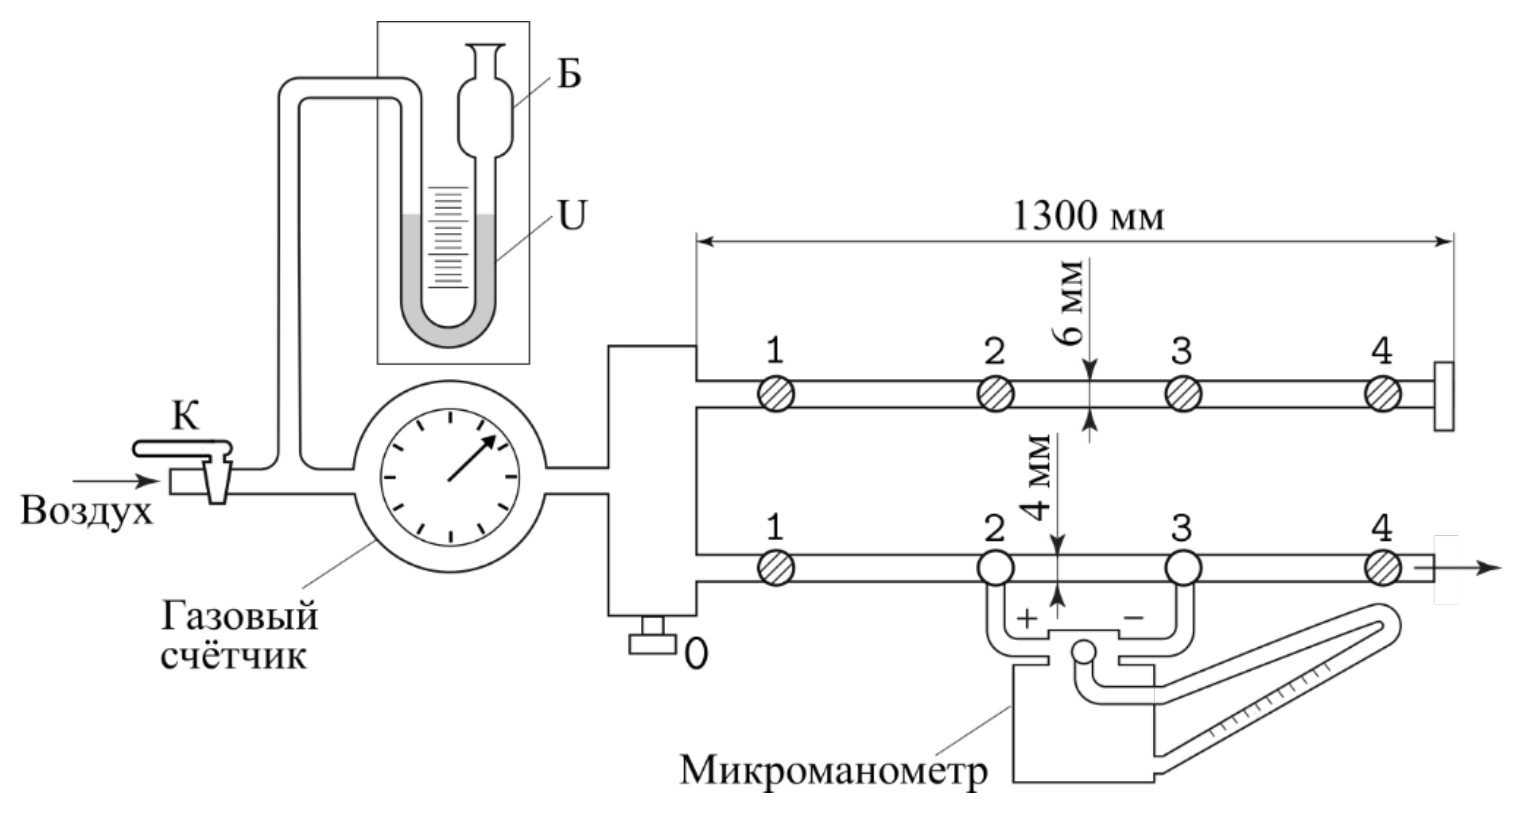
\includegraphics[width=0.8\linewidth]{img/eq1.png}
\end{figure}

Схема установки приведена на рисунке. Поток воздуха под давлением, немного превышающем
атмосферное, поступает через газовый счетчик в тонкие металлические трубки. 
Воздух нагнетается компрессором, интенсивность его подачи регулируется краном К. Трубки
снабжены съемными заглушками на концах и рядом миллеметровых отверстий, к которым
можно подключать манометр. В рабочем состоянии открыта заглушка на одной трубке,
микроманометр подключен к двум ее выводам, а все остальные отверстия плотно закрыты
пробками.

Перед входом в газовый счетчик установлен водяной манометр. Он служит для измерения
давления газа на входе, а также предохраняет счетчик от выхода из строя.

В работе используются газовый счетчик, основанный на принципе вытеснения и
микроманометр. Разность давлений на входах манометра измеряется по высоте подъема рабочей
жидкости. Регулировка наклона позволяет измерить давление в различных диапазонах.
